\documentclass{article}
\usepackage[utf8]{inputenc}
\usepackage[spanish]{babel}
\usepackage{listings}
\usepackage{graphicx}
\usepackage{geometry}
\graphicspath{ {images/} }
\usepackage{cite}

\geometry{
textheight=23cm}
\begin{document}

\begin{titlepage}
    \begin{center}
        \vspace*{1cm}
            
        \Huge
        \textbf{INFORMA2 S.A.S}
            
        \vspace{0.5cm}
        \LARGE
        Parcial 2: Implementación
            
        \vspace{5cm}
            
        \textbf{Juan Pablo Cruz Gómez}
        
        \vspace{0.5cm}
        
        \textbf{Erika Dayana León Quiroga}
            
        \vfill
            
        \vspace{0.8cm}
            
        \Large
        Despartamento de Ingeniería Electrónica y Telecomunicaciones\\
        Universidad de Antioquia\\
        Medellín\\
        Septiembre de 2021
            
    \end{center}
\end{titlepage}

\tableofcontents
\newpage
\section{Sección introductoria}\label{intro}
En este informe se mostrará y explicará la implementación del problema presentado en el Parcial 2 de la materia Informática II

\section{Clases implementadas} \label{clases}

\subsection{Citación}



\section{Módulos del código implementado} \label{Modulos}

\section{Estructura del circuito} \label{circuito}

\begin{figure}[h]
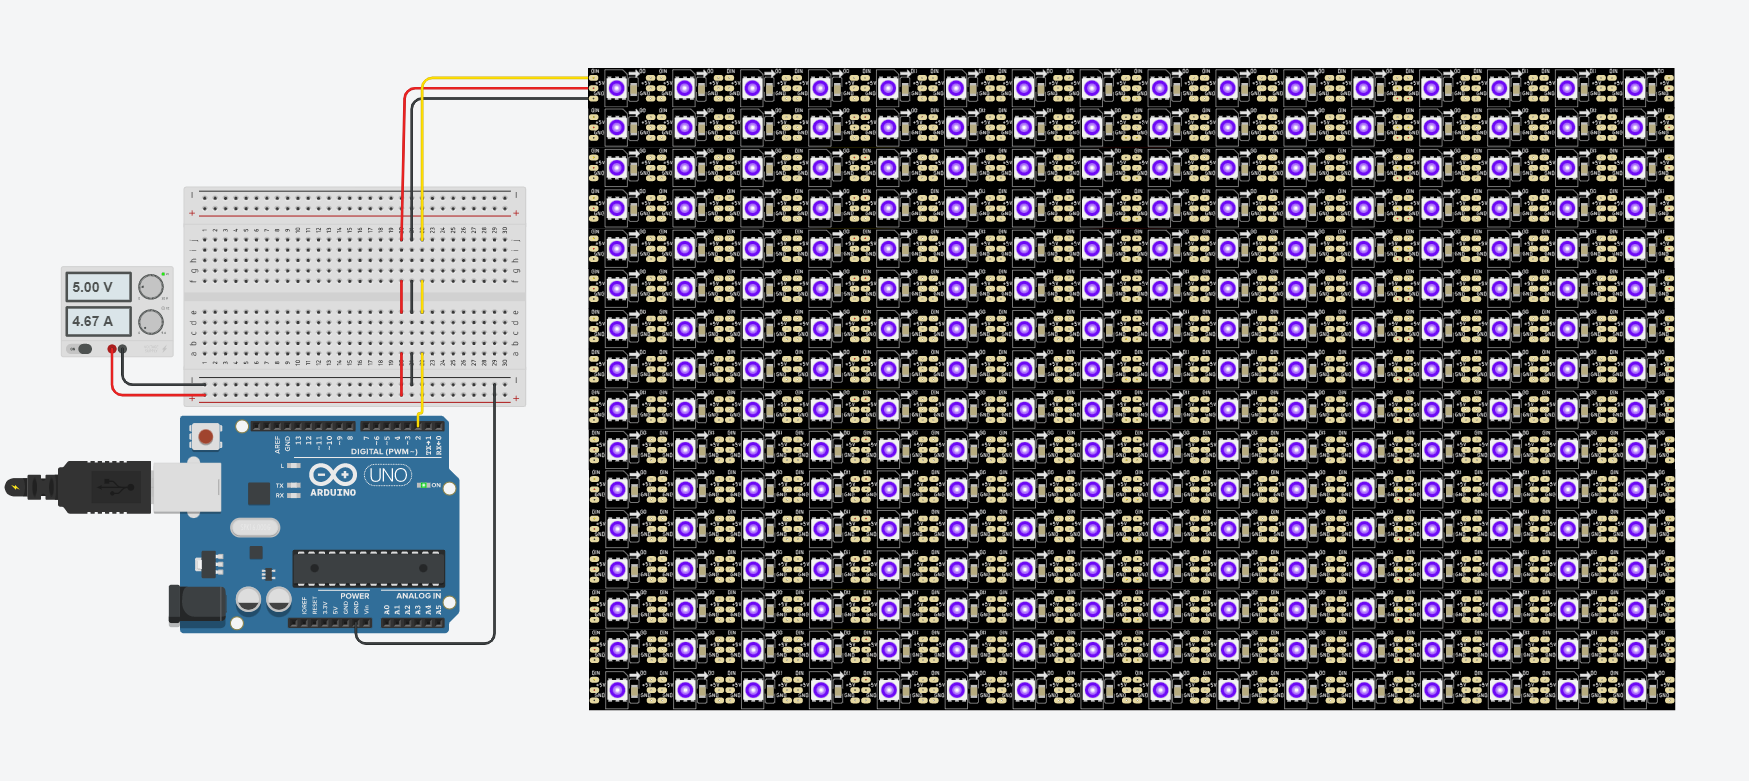
\includegraphics[width=15cm]{LEDs16x16.png}
\centering
\caption{Montaje de la matriz de LEDs de 16x16}
\label{fig:punto1}
\end{figure}


\section{Problemas presentados} \label{problemas}

\end{document}
